\documentclass[oneside,openany]{memoir}
\usepackage{lmodern}
\usepackage{amssymb,amsmath}
\usepackage{mathtools}
\usepackage{ifxetex,ifluatex}
\usepackage{fixltx2e} % provides \textsubscript
\ifnum 0\ifxetex 1\fi\ifluatex 1\fi=0 % if pdftex
  \usepackage[T1]{fontenc}
  \usepackage[utf8]{inputenc}
\else % if luatex or xelatex
  \ifxetex
    \usepackage{mathspec}
    \usepackage{xltxtra,xunicode}
  \else
    \usepackage{fontspec}
  \fi
  \defaultfontfeatures{Mapping=tex-text,Scale=MatchLowercase}
  \newcommand{\euro}{€}
\fi
% use upquote if available, for straight quotes in verbatim environments
\IfFileExists{upquote.sty}{\usepackage{upquote}}{}
% use microtype if available
\IfFileExists{microtype.sty}{\usepackage{microtype}}{}
\usepackage{longtable,booktabs}
\usepackage{graphicx}
\makeatletter
\def\maxwidth{\ifdim\Gin@nat@width>\linewidth\linewidth\else\Gin@nat@width\fi}
\def\maxheight{\ifdim\Gin@nat@height>\textheight\textheight\else\Gin@nat@height\fi}
\makeatother
% Scale images if necessary, so that they will not overflow the page
% margins by default, and it is still possible to overwrite the defaults
% using explicit options in \includegraphics[width, height, ...]{}
\setkeys{Gin}{width=\maxwidth,height=\maxheight,keepaspectratio}
\ifxetex
  \usepackage[setpagesize=false, % page size defined by xetex
              unicode=false, % unicode breaks when used with xetex
              xetex]{hyperref}
\else
  \usepackage[unicode=true]{hyperref}
\fi
\hypersetup{breaklinks=true,
            bookmarks=true,
            pdfauthor={Michele Pittoni},
            pdftitle={Advanced Topology Analysis in Three Wireless Community Networks},
            colorlinks=true,
            citecolor=blue,
            urlcolor=blue,
            linkcolor=magenta,
            pdfborder={0 0 0}}
\urlstyle{same}  % don't use monospace font for urls
\usepackage[normalem]{ulem}
% avoid problems with \sout in headers with hyperref:
\pdfstringdefDisableCommands{\renewcommand{\sout}{}}
\setlength{\parindent}{0pt}
\setlength{\parskip}{6pt plus 2pt minus 1pt}
\setlength{\emergencystretch}{3em}  % prevent overfull lines
\setcounter{secnumdepth}{0}

\title{Advanced Topology Analysis in Three Wireless Community Networks}
\author{Michele Pittoni}
\date{2014 - VI}

\begin{document}
\maketitle

\newcommand{\st}{\text{ st. }}
\newcommand{\etx}{\mathrm{ETX}}
\newcommand{\linkq}{\mathrm{LQ}}
\newcommand{\nlq}{\mathrm{NLQ}}
\newcommand{\mpr}{\mathrm{MPR}}

\chapterstyle{section}

\chapter*{Introduction}\label{introduction}
\addcontentsline{toc}{chapter}{Introduction}

Wireless Community Networks (WCNs), a particular kind of wireless mesh
networks, have become more and more popular in recent years. These
networks are different from traditional ones in various aspects, such as
the link nature and the arising topologies. For this reason, generic
network protocols may not be well suited for WCNs and much research
effort is being dedicated to the development of new routing protocols
for this networks and for measuring their efficiency.

This works provides an introduction to the topic of Wireless Community
Networks and a description of the three networks which are subsequently
analysed. Also provided is an introduction to OLSR, the routing protocol
which is used in the analysed networks. The biggest part focuses on the
analysis of some efficiency metrics for the chosen networks and a
comparison with some well known random network models.

\chapter{Wireless Community Networks}\label{wireless-community-networks}

The phrase ``Wireless Community Network'' has been used in literature to
indicate various kinds of projects. The most common usage refers to
wireless mesh networks operated by a community of citizens, as opposed
to those controlled by a single entity (corporation or government).
Other authors also use the term for the public hotspot networks run by
municipalities, or more generally for networks that provide wireless
connection to the public. In this document the term is used with the
first meaning, only for networks which are run -- not merely accessible
-- by the community.

\section{History}\label{history}

The appearence of the first Wireless Community Networks can be dated to
the late 1990s-early 2000s, when the IEEE 802.11 protocol (WiFi) was
first introduced. They started as experiments by radio enthusiasts who
wanted to explore the potential of this new technology, pushing it to
the limit: WiFi was designed as a protocol for local communication, but
it was shown that, with the right equipment, it can perform well also on
long distance links. The experimentation was made easier by the
unlicensed spectrum of frequencies in which WiFi operates.

With WiFi gaining popularity and wireless enabled devices becomnig
mainstream, the cost of WiFi equipment decreased and so did the barrier
to participate in WCNs. At the same time, wireless protocols evolved and
improved -- for example 802.11a worked in the less crowded 5GHz band,
allowing more separation between the used frequencies and thus less
interference. In addition, a key factor to the diffusion on WCNs was the
scarce availability of broadband connections in certain areas. In such
cases, networks were not an experiment anymore, but were used to provide
services where commercial initiatives were lacking.

Today, the WCN scenario is varied: in some places they are used to
mitigate the digital divide, elsewhere they remaind experimental
testbeds or are more focused on the social/political aspect of being an
autonomous network owned and run by citizens. In the latter, the focus
is on the services provided inside the network rather than on Internet
access, even if it may be available. Some WCNs have grown to the point
of having an Autonomous System (AS) number assigned and being able to
peer with other networks at Internet eXchange Points (IXPs).

WCNs usually have a cultural background of Open Source enthusiasts and
hackers\footnote{as in ``curious'', not as in ``criminal''} in general.
Some of them are run by a formal associations, other by informal groups
of citizens, but in every case node owners know each other and there is
a sense of community. More experienced participants share their
technical knowledge (and their time), making it possible for new members
to enter the network with minimum effort.

Because of their nature of not asking permissions, it is difficult to
determine precisely the number of active WCNs as there is no central
registry to look at. However, there is a Wikipedia page\footnote{(``List
  of Wireless Community Networks by Region. Wikipedia, the Free
  Encyclopedia'' 2014)} which, albeit incomplete, lists 262 WCNs at the
time of writing. The dimensions of such networks are varied, from just a
handful of nodes to nearly 25,000 as in Guifi\footnote{\url{http://guifi.net}},
which is widely regarded as the world's largest WCN.

\section{Technology}\label{technology}

\begin{figure}[htbp]
\centering
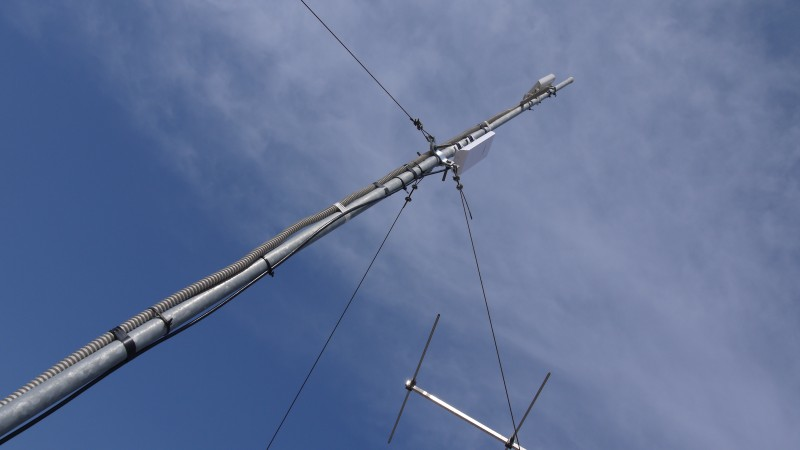
\includegraphics{images/ninux_node.png}
\caption{Antennas of a WCN node}
\end{figure}

WCNs were born together with the IEEE 802.11 protocol family and
continue to use it for various reasons, such as hardware availability
and low cost, unlicensed frequency spectrum operation and the constant
improvement of subsequent versions. Other solutions for the pyhsical
layer are sometimes used -- for example proprietary protocols, maybe
operating in licensed frequencies, or even methods not based on
radio\footnote{Ronja, \url{http://ronja.twibright.com/}} -- but they are
an uncommon last resort when WiFi can not work (due to interference or
other reasons).

A node of a WCN is a router connected with one or more radio interfaces.
There is not a standard for the construction of a node, but over time
every community has gathered some best practices and guidelines based on
experience and trial-and-error. The equipment used varies from consumer
WiFi routers (such as the very popular Linksys WRT54GL) with homemade
antennas, to professional and more expensive equipment dedicated to
long-range WiFi links. Smaller nodes, especially if they are near enough
to other ones, may use a single omnidirectional antenna to connect to
different nodes. Usually, however, directional antennas with a limited
beam width are used, to reduce interference leveraging different
channels, avoid receiving noise from all directions and achieve an
higher gain. Some nodes use both kinds of antennas, directional for
backbone links and omnidirectional to provides an hotspot access.

\begin{figure}[htbp]
\centering
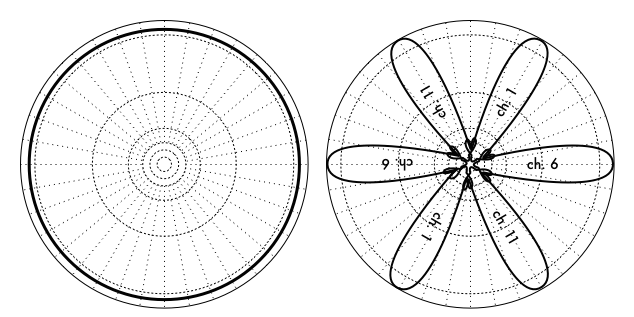
\includegraphics{./images/directional-antennas.png}
\caption{The difference between an omnidirectional and multiple
monodirectional antennas.}
\end{figure}

Routing is one of the biggest challenges in wireless mesh networks. Due
to the very nature of wireless links, traditional routing protocols
thought for wired networks perform poorly when applied to them. In
recent years, many new routing protocols have been proposed to address
this issue and today there is a competition with no clear winner. The
two most widely known routing protocols for wireless mesh and ad-hoc
networks are OLSR and BATMAN. The former, which is used in the three
WCNs analysed in this work, will be the subject of chapter 3. \emph{some
words on BATMAN?}

\chapter{Network topology and graphs}\label{network-topology-and-graphs}

Some mathematical instruments are required to do any kind of description
or analysis of the topology of a network, or to explain the functioning
of a routing protocol.

The mathematical structure which is used to describe networks is the
graph. A \emph{simple, undirected graph} is an ordered pair
$G = (V, E)$, where elements of $V$ are the \emph{nodes} (also called
\emph{vertices}) of the graph and are usually denoted with letters
$u,v,w,\ldots$, while $E \subseteq \binom{V}{2}$ is the set of the
\emph{edges} of the graph. For convenience,
$e_{ij} \coloneqq \{v_i, v_j\} \in E$.

An edge $e_{ij}$ is said to be \emph{incident} to the vertices $v_i$ and
$v_j$; equivalently, $v_i$ and $v_j$ are incident to $e_{ij}$. Two
vertices incident to the same edge are said \emph{adjacent}.

The graph is said simple since there are no loops (i.e.
$\{u,u\} \not\in E$) and each pair of vertices is connected by at most
one edge. The above mentioned graph is also said undirected. On the
other hand, a \emph{directed graph} is a pair $D = (V, A)$ where
$A = \{(u,v) | u,v \in V,\, u \neq v\}$ -- the elements of $A$ are
usually called \emph{arcs}.

For the purposes of describing networks, graphs are considered to be
\emph{finite}, so $N$ and $E$ are finite sets. Many well known finite
graph properties do not hold in the infinite case.

A \emph{weighted graph} is a graph in which every edge has an associated
label \emph{weight}, usually a real number. It is useful to define a
function $w: E \rightarrow \mathbb{R}$ which associates weights to
edges; in the case of unweighted graphs, it can be assumed
$w: e \mapsto 1\, \forall e \in E$.

To model networks as graphs, each node of the network is represented by
a node in the graph and a link between two nodes is represented by an
edge between those nodes. If there are unidirectional link, a directed
graph is used. For the purposes of this work, every link is considered
bidirectional and symmetric, so from now on ``graph'' will be use for
simple, undirected graphs.

\section{Terminology}\label{terminology}

\subsection{Order and size}\label{order-and-size}

The \emph{order} of a graph is the number of its nodes, $|V|$. The
\emph{size} of a graph is the number of its edges, $|E|$.

\subsection{Degree}\label{degree}

The \emph{degree} $k_v$ of a vertex $v$ is the number of edges incident
to that vertex. A vertex of degree 0 is an \emph{isolated vertex}. A
vertex of degree 1 is a \emph{leaf}.

The \emph{total degree} of a graph is $\sum_{v \in V} k_v$.

The \emph{degree sequence} of a graph is the list of degrees in
non-increasing order. Not every non-increasing sequence of integers is
the degree sequence of some graph.

The \emph{degree distribution} of a graph is a function
$p_k: \mathbb{N} \rightarrow [0, 1]$ such that

\begin{equation*}
p_k(n) = \frac{\left\vert{ \{v \in V \st k_v = n\} }\right\vert}{|V|}
\end{equation*}

The degree distribution is a discrete probability distribution since
$\sum_{k} p_k = 1$.

\subsection{Subgraphs}\label{subgraphs}

A \emph{subgraph} $G' = (V', E')$ of $G$ is a graph such that
$V' \subseteq V$ and $E' \subseteq E\restriction_{V'}$, where
$E\restriction_{V'} = \{\{v_i, v_j\} \in E \st v_i,v_j \in V'\}$.

\subsection{Walks, paths}\label{walks-paths}

A \emph{walk} is a sequence of vertices
$P = (v_0, v_1, \ldots, v_n) \in V \times V \times \ldots \times V$ such
that $e_ij \in E,\, 0 \leq i < n$. A walk is \emph{closed} if
$v_0 = v_n$, \emph{open} otherwise. The \emph{length} of the walk is
$n$. The \emph{weight} of the walk is $w_P = \sum_0^{n-1} w(e_ij)$. In
unweighted graphs, $w_P = N$.

A \emph{path} is a walk with no repeated vertices. A \emph{cycle} is a
closed walk with no repeated vertices, except obviously the starting one
which is repeated once at the end.

Given a graph with no negative-weight cycles, a \emph{geodesic path},
also called \emph{shortest path}, between $v_0$ and $v_n$ is a walk
$P = (v_0, v_1, \ldots, v_n)$ such that
$\nexists P' = (u_0, u_1, \ldots, u_m)$ with
$u_0 = v_0,\, u_m = v_n \st w_{P'} < w_P$. Note that $P$ is a path: if
$\exists v_i, v_j \in P \st v_i = v_j$, then
$\exists P' = (v_0, \ldots, v_i, v_{j+1}, \ldots, v_n) \st w_{P'} < w_P \Rightarrow P$
is not the geodesic path.\\In a graph with negative-weight cycles, the
geodesic path is not defined, since it is possible to have walks with
$w_P = -\infty$.\\The length of a geodesic path (which is the length of
all of them) from $u$ to $v$ is called \emph{geodesic distance} of $u$
and $v$, indicated with $d_{uv}$

\subsection{Neighbours}\label{neighbours}

Each vertex adjacent to $v$ is also called a \emph{neighbour} of $v$.
The set of the neighbours of $v$ is called \emph{neighbourhood} of $v$.

The concept of neighbourhood may be extended to vertices at any
distance. For example, the \emph{2-hop neighbourhood} of $v$ is the set
of vertices $u$ such that there is a walk from $v$ to $u$ whit lenght 2.
Similarly, the \emph{strict 2-hop neighbourhood} of $v$ is the set of
vertices which are in the 2-hop neighbourhood, excluding $v$ itself and
its direct neighbours.

\subsection{Connectivity}\label{connectivity}

A graph is called \emph{connected} if, for each pair $\{u,v\}$ of nodes,
there is a path between $u$ and $v$.

A \emph{connected component} of $G$ is a maximally connected subgraph of
$G$.

\subsection{Centrality}\label{centrality}

In network science there is substantial interest in the concept of the
centrality of a vertex (or an edge) in a graph. The idea behind this
metric is to determine the most ``important'' components of a network.
The meaning of ``important'' varies depending on the context: in social
networks importance is usually defined by the influence of a node,
measured by the size of it neighbourhood. In communication networks, the
most important nodes are those who participates most communications,
either by forming circuits or by relaying packets. These are just two
examples of different notions of importance that require different ways
to be measures. In the following paragraphs, the centrality metrics
relevant to this work are presented.

\subsubsection{Degree centrality}\label{degree-centrality}

The degree of a vertex is the simplest possible measure of centrality
and it is the only one that is only based on local properties. This is
an advantage from the computational point of view, but it also implies
that degree centrality is the least significant centrality metric.
Nonetheless, depending on the graph, it can approximate quite well the
behaviour of other metrics.

\begin{equation}
C_D(v) = k_v
\end{equation}

\subsubsection{Betweenness centrality}\label{betweenness-centrality}

Betweenness centrality of vertex $v$ is defined as the fraction of
shortest paths between any two vertices that pass through $v$. Formally,
define $\sigma(s,t)$ the number of shortest paths from $s$ to $t$ and
$\sigma(s,t|v)$ the number of those paths that pass through $v$. If
$s = t,\, \sigma(s,t) = 1$. There is not a consensus in literature if a
path ``passes through'' its endpoint; in this case, it is assumed not:
$\sigma(s,t|s) = \sigma(s,t|t) = 0$. The betweennes centrality is

\begin{equation}
C_B(v) = \sum_{s,t \in V} \frac{\sigma(s,t|v)}{\sigma(s,t)} %_
\end{equation}

Betweennes centrality is especially useful in the study of communication
networks because information usually travels through the shortest path,
so $C_B$ helps estimating how much traffic a node will see, in a way
other centrality measures do not consider. For example, in the classic
Barbell graph -- two complete graphs connected by a path -- vertices on
the path have a very small degree but since every path between the two
complete graphs passes through them they have high betweenness. This
reflects the big control they have over the communications between other
nodes.

\subsubsection{Edge betweenness
centrality}\label{edge-betweenness-centrality}

The concept of betweenness centrality can also be easily extended to
edges, with a similar notation.

\begin{equation}
C_{E}(e) = \sum_{s,t \in V} \frac{\sigma(s,t|e)}{\sigma(s,t)}
\end{equation}

\subsubsection{Closeness centrality}\label{closeness-centrality}

Closeness centrality is also based on shortest paths, but has a
different approach and a different meaning. It is based on the mean
distance between $v$ and the other vertices. If $d_{vu}$ is the geodesic
distance between $v$ and $u$, the \emph{mean geodesic distance} from $v$
to $u$, averaged over all vertices $u$ is

\begin{equation}
\mathcal{L}_v = \frac{1}{n} \sum_u d_{vu}  %_
\end{equation}

Since usually centrality measures have high values for more central
nodes, closeness centrality is usually defined as the inverse of the
mean distance $\mathcal{L}_v$.

\begin{equation}
C_C(v) = \frac{1}{\mathcal{L}_v} = \frac{n}{\sum_u d_{vu}}  %_
\end{equation}

Closeness centrality, despite being often used in network studies, has
come shortcomings. For example, the above definition is only valid if
the graph is connected, since $d_{vu}$ is defined to be infinite if
there is no path from $v$ to $u$. In graphs with more than one connected
components, $C_C$ would then be zero for every vertex. The usual
solution is to compute the closeness centrality for each connected
component separately: this works, but since distances are usually
smaller in small components, vertices in those components tend to have
higher closeness centrality, which may be undesirable.

Another issue with closeness centrality is that its values are often
cramped in a small range from lowest to highest. In most networks
distances tend to be small, typically increasing with the logarithm of
the size $n$ of the graph. So, the lower and upper bound for
$\mathcal{L}_v$ are, respectively, $1$ and $\log n$. Similarly, the
range for $C_C$ is limited.

\section{Random graph models}\label{random-graph-models}

A random graph is a graph generated by a random process. The reason for
using random graph models in network analysis is that they can produce
graphs with known degree distributions, which can be used to prove
mathematically or otherwise analyse empirically their structural and
dynamical properties.

\subsection{Erd\H{o}s-Rényi random
graph}\label{erds-ruxe9nyi-random-graph}

The random graph model originally proposed by Erd\H{o}s and Rényi is
also called $G(n,M)$ model, since it consists in the uniform random
selection of a graph from the set of all graphs with $n$ nodes and $M$
edges.

The model used here is a variaton first introduced by (Gilbert 1959),
called the $G(n,p)$ model. The algorithm starts form a graph with $n$
nodes and no edges. Then, for each unordered pair of nodes
$\{i,j\} . i \neq j$, the edge $ij$ is added with probability $p$.

The $G(n,p)$ models has some interesting properties which are not
obvious at a first look. For example, the number of edges is not known
as in the $G(n,M)$ models, but the expected number of edges can be
determined to be $\binom{n}{2}p$. Another important aspect is
connectedness: for $p > \frac{(1+\epsilon) \ln n}{n}$ the graph will
almost surely be connected, while for $p < \frac{(1-\epsilon) \ln n}{n}$
it will almost surely have isolated vertices.

Finally, the degree distribution has the form

\begin{equation}
p_k = \binom{n-1}{k} p^k (1-p)^{n-1-k}
\end{equation}

\subsection{Barabási-Albert graph}\label{barabuxe1si-albert-graph}

A scale free network is a network whose degree distribution follows a
power law of the form

\begin{equation}
p_k = Ck^{-\alpha}
\end{equation}

A method for generating graphs with a power law degree distribution,
using a preferential attachment mechanism, was devised by A. L. Barabási
and R. Albert in (Barabási and Albert 1999). This is the method
implemented by NetworkX. Given a target number $n$ of nodes and a
parameter $m$ which controls the density of the network, the algorithm
starts from a graph with $m$ nodes and no edges. Then other nodes are
added and from each new node $m$ edges are created. The new edges are
attached preferentially to the nodes with higer degree. This continues
until there are $n$ nodes in the graph, meaning the final graph will
contain $(n-m) m$ edges.

\chapter{OLSR summary}\label{olsr-summary}

Optimized Link State Routing (OLSR) is a proactive routing protocol
standardized by the IETF in RFC 3626\footnote{Clausen and Jacquet (2003)}
and designed to have a better performance on wireless mesh and ad-hoc
networks than traditional protocols for wired networks.

In link state routing protocols, each node is supposed to know the
entire topology of the network in order to calculate the routes. This
means that each time the topology changes, the new information must be
propagated to every node. This is traditionally done by flooding
link-state advertisement packet through the network.

In the case of traditional networks with wired links, this method is
acceptable since the topology seldom changes. In WCN (and wireless
networks in general), however, links change their cost quite often and
may also disappear temporarily. Flooding in this situation imposes a big
effort on the network and may degrade the performance consistently.

OLSR addresses this concern with an optimized flooding mechanism which
significantly reduces the overhead by using only selected nodes, called
multipoint relays (MPRs), to broadcast link-state advertisements. The
next sections outline the details of this mechanism and of OLSR in
general.

\begin{figure}[htbp]
\centering
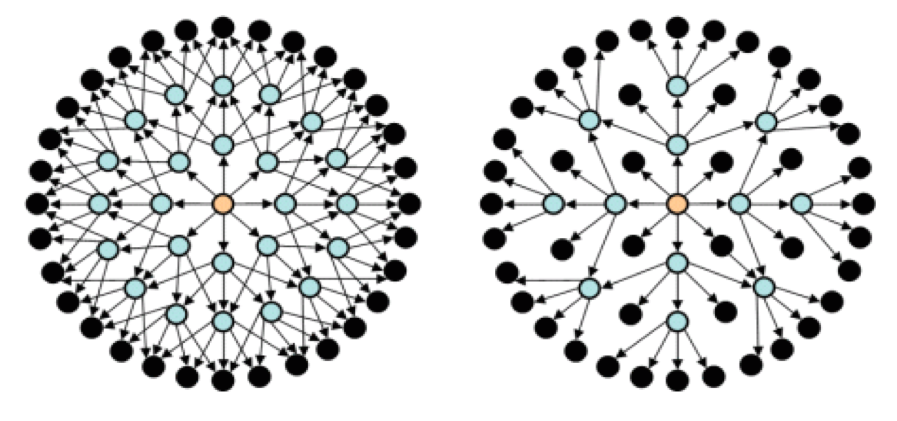
\includegraphics{images/mpr.png}
\caption{Flooding vs.~MPR forwarding}
\end{figure}

\section{Generic packet format}\label{generic-packet-format}

OLSR uses different types of messages in its specification. In order to
take advantage of the maximal frame size provided by the network, one or
more messages are encapsulated in a packet which has the same format for
all types of messages. This facilitates the extensibility of the
protocol and allows the transmission of different kinds of information
in a single packet.

Each message is flooded through the network with a TTL. The transmission
to neighbours is just a special case of flooding. Duplication is
eliminated locally, since each node maintains a set of messaged it has
already processed, and minimized globally by the MPR mechanism.

\begin{verbatim}
 0                   1                   2                   3
 0 1 2 3 4 5 6 7 8 9 0 1 2 3 4 5 6 7 8 9 0 1 2 3 4 5 6 7 8 9 0 1
+-+-+-+-+-+-+-+-+-+-+-+-+-+-+-+-+-+-+-+-+-+-+-+-+-+-+-+-+-+-+-+-+
|        Packet Length          |    Packet Sequence Number     |
+-+-+-+-+-+-+-+-+-+-+-+-+-+-+-+-+-+-+-+-+-+-+-+-+-+-+-+-+-+-+-+-+
|  Message Type |     Vtime     |         Message Size          | 
+-+-+-+-+-+-+-+-+-+-+-+-+-+-+-+-+-+-+-+-+-+-+-+-+-+-+-+-+-+-+-+-+
|                      Originator Address                       |
+-+-+-+-+-+-+-+-+-+-+-+-+-+-+-+-+-+-+-+-+-+-+-+-+-+-+-+-+-+-+-+-+
|  Time To Live |   Hop Count   |    Message Sequence Number    |
+-+-+-+-+-+-+-+-+-+-+-+-+-+-+-+-+-+-+-+-+-+-+-+-+-+-+-+-+-+-+-+-+
|                                                               |
:                            MESSAGE                            :
|                                                               |
+-+-+-+-+-+-+-+-+-+-+-+-+-+-+-+-+-+-+-+-+-+-+-+-+-+-+-+-+-+-+-+-+
|  Message Type |     Vtime     |         Message Size          | 
+-+-+-+-+-+-+-+-+-+-+-+-+-+-+-+-+-+-+-+-+-+-+-+-+-+-+-+-+-+-+-+-+
|                      Originator Address                       |
+-+-+-+-+-+-+-+-+-+-+-+-+-+-+-+-+-+-+-+-+-+-+-+-+-+-+-+-+-+-+-+-+
|  Time To Live |   Hop Count   |    Message Sequence Number    |
+-+-+-+-+-+-+-+-+-+-+-+-+-+-+-+-+-+-+-+-+-+-+-+-+-+-+-+-+-+-+-+-+
|                                                               |
:                            MESSAGE                            :
|                                                               |
+-+-+-+-+-+-+-+-+-+-+-+-+-+-+-+-+-+-+-+-+-+-+-+-+-+-+-+-+-+-+-+-+
:                                                               :
               (etc.)
\end{verbatim}

\section{Link sensing and neighbour
discovery}\label{link-sensing-and-neighbour-discovery}

MPRs are selected locally by each node between its neighbours. The
requirement is that the MPRs of a node $v$ must cover, with the union of
their neighbourhoods, the 2-hop neighbourhood of $v$. Thus, in order to
select its MPRs, a node must know its 2-hop neighbours and how to reach
them.

The message type used in OLSR for this purpose is the \texttt{HELLO}
message, which is transmitted by each node to its neighbours and
contains the addresses of the neighbour it knows. Of course, the first
\texttt{HELLO} messages are empty and only serve the purpose of link
sensing. After each node populates its neighbour set, it includes this
information in its \texttt{HELLO} messages, along with some information
on the links and the neighbours (e.g.~if the links are verified to be
symmetric). This allows all nodes to gather the necessary knowledge of
their 2-hop neighbourhood.

\texttt{HELLO} messages are generated and transmitted at a regular
interval (\texttt{HELLO\_INTERVAL}). Lost links are also advertised for
some time (with a link type of \texttt{LOST\_LINK}).

\section{MPR selection and
signalling}\label{mpr-selection-and-signalling}

Using the information from the \texttt{HELLO} messages, each node can
select a set of its neighbours such that every node in its 2-hop
neighbourhood is at 1 hop from the set. Formally, call $N_1(u)$ the
neighbourhood, $N_2(u)$ the strict 2-hop neighbourhood, select
$\mpr(u) \subseteq N_1(u)$ such that

\begin{equation*}
%*
\forall v \in N_2(u) \. \exists s \in \mpr(u) \text{ st. } v \in N_1(s)
\end{equation*}

This requirement essentially means that each node in the strict 2-hop
neighbourhood can be reached through a MPR. The protocol specification
suggests that the MPR set of each node should be as small as possible,
but does not require it. Once a node has selected its MPRs, it needs to
signal its choice to the neighbours, so that the selected nodes know
that they must retransmit its broadcasts (and the other nodes know not
to do that). \texttt{HELLO} messages are used also for this purpose: the
selected MPRs are advertised with a neighbour type of
\texttt{MPR\_NEIGH}.

\section{Message forwarding}\label{message-forwarding}

Observing the \texttt{HELLO} messages it receives, each node populates
and maintains an \texttt{MPR Selector Set}. This is the set of nodes
that selected it as an MPR or, in other words, the set of nodes whose
transmissions are to be forwarded by the node in question.

When a node receives a message (except for \texttt{HELLO} messages,
which are never forwarded), it checks if the time-to-live has reached
zero or if the message was already processed (by examining the duplicate
set). If the message passes this preliminary checks, it is forwarded
only if it was received from a selector.

This strategy obviously reduces the number of times a single message is
forwarded. Thanks to the construction of the MPR set, the strategy also
ensures that each message can reach every node in the network.

\section{Topology control}\label{topology-control}

The link-state information is propagated throughout the network with
\texttt{Topology Control} messages (\texttt{TC}). This messages are
generated only by the nodes which have been selected as MPR for some
other node and propagated following the above described rules. Each
\texttt{TC} message contains the identification of the node who
generated the message and a list of the addresses of some of its
neighbours.

The OLSR specification requires that the nodes in the
\texttt{MPR Selector Set} of a node be in the \texttt{TC} messages it
generates. To add redundancy, each node can advertise, in addition, the
neighbours selected by it as MPRs, or even all of its neighbours. The
added redundancy comes at the cost of longer \texttt{TC} messages, which
may be more susceptible to congestion.

\section{Link quality}\label{link-quality}

OLSR implements a mechanism to avoid using ``bad'' links (i.e.~links
which are usually too weak but may let \texttt{HELLO} messages pass from
time to time). Since \texttt{HELLO} messages are transmitted at a
regular interval, each node knows how many of them to expect from each
neighbour over a period of time. Comparing this with the number of
received messages it computes a measure of the Link Quality (LQ). This
metric was originally only used to decide if a link was reliable enough
to use. New versions of OLSR have put more importance on link quality.

It is common in WCNs to use the ETX metric to express link quality. ETX
stands for Expected Transmission Count and was proposed in De Couto
(2004). It indicates the expected number of transmissions (including
retransmissions) required to successfully deliver a packet.

In OLSR, ETX is derived directly from LQ. \texttt{HELLO} messages
contain the calculated values, so each node has for every link two
measures: its own (LQ) and its neighbour's (NLQ). Since each packet
transmission requires an acknowledgement, the estimated probability of
success is $\linkq \cdot \nlq$. ETX is calculated as

\begin{equation}
\etx = \frac{1}{\linkq \cdot \nlq}
\end{equation}

\chapter{The analysed networks}\label{the-analysed-networks}

The three WCNs which are analysed later are Ninux, Funkeuer Wien and
Funkfeuer Graz. The study considers 50 snapshots of the networks taken
from \ldots{} to \ldots{} .

\section{Ninux}\label{ninux}


\includegraphics{images/ninux_logo.png} Ninux\footnote{\url{http://wiki.ninux.org/}}
is the largest italian WCN. It was started in 2001 in Rome and now
consists of about 250 active nodes, located in different ``Ninux
islands'' all over Italy. The name ``Ninux'' originally was a tribute to
the project founder, Nino, but now the project members usually take it
with the meaning ``Neighbourhood Internet, Network Under eXperiment''.

Ninux is managed in an informal way: every member is the owner and
responsible of its node (or nodes), but there is no formal association.
This is a deliberate choice of the Ninux community, motivated by the
excessive bureaucratic effort it would require. Moreover, all
associations must have a president responsible for the activities of the
association itself, and Ninux members prefer the responsibility to be
decentralised (as the network is).

The different islands use a variety of protocols and have different
topologies:

\begin{itemize}
\itemsep1pt\parskip0pt\parsep0pt
\item
  in Pisa, Sicily and Friuli there are three mesh networks, with routing
  based on B.A.T.M.A.N.
\item
  in Rome, the biggest Ninux island uses a backbone with point-to-point
  links combined with some mesh areas, employing OLSR for all the
  routing
\item
  in recent years other networks have been created in Florence, Viterbo,
  Catanzaro, Cosenza and Reggio Calabria, all based on OLSR
\end{itemize}

The islands are connected together by tunnels using a variety of
protocols.

Ninux is an Autonomous System (AS\# 197835)\footnote{\url{https://apps.db.ripe.net/search/query.html?searchtext=AS197835\&object_type=aut-num\#resultsAnchor}}
and it is a member of the NaMeX\footnote{\url{http://www.namex.it/en/who/members}}
Internet Exchange Point.

In this work, the biggest Ninux island has been analyzed (since it is
the biggest OLSR routing domain), which is Rome's newtork. It consists
of 132 nodes connected by 154 links (average degree of 2.333).

\begin{figure}[htbp]
\centering
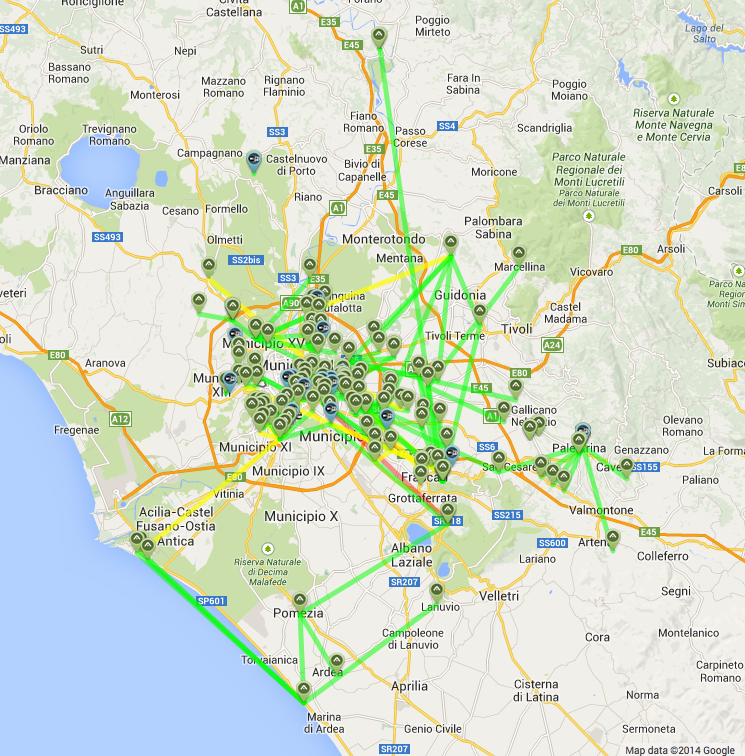
\includegraphics{images/ninux_map.png}
\caption{Map of the Rome Ninux island}
\end{figure}

\section{FunkFeuer: Wien}\label{funkfeuer-wien}

FunkFeuer\footnote{\url{http://www.funkfeuer.at/}} is a project that
comprises networks in different parts of Austria (Vienna, Graz, parts of
Weinviertel and Bad Ischl). The literal meaning of ``funkfeuer'' in
german is ``radio beacon''. FunkFeuer is also a registered association
in Austria, differently from Ninux.

The origins of FunkFeuer are in the experiments of an austrian ISP based
in Vienna, Silver Server, which, during the 1990s, explored the
commercial viability of wireless radio data links. After a test phase,
Silver Server ultimately decided that the technology was not ready to be
used commercially; however, the infrastructure was already in place and
it was handed off to two associations, Team Teichenberg and Public Voice
Lab. With direction from Franz Xaver and Roland Jankowski, they further
expanded the network, bringing the node count to 15, but failed to
create easy end-user access.

The network was ultimately decentralised, giving the opportunity to the
citizens to buy the hardware of the nodes. The advent of cheap GNU/Linux
based embedded WiFi products promoted the growth of the network and an
association was founded to have a more structured organisation and
address the issues of decentralisation. The existence of a formal
association also enables to request sponsoring from local
administrations.

FunkFeuer Wien (FFWien)\footnote{\url{http://www.funkfeuer.at/Vienna.206.0.html?\&L=1}}
is the biggest of FunkFeuer networks, covering 1/3 of the city. The
active node in the analysed snapshots were 237, with 433 links (an
average degree of 3.654).

\section{FunkFeuer: Graz}\label{funkfeuer-graz}

FunkFeuer Graz (FFGraz)\footnote{\url{http://graz.funkfeuer.at/}} is the
``smaller sister'' of the FFWien network, situated in the homonymous
city. It was founded after FFWien by Othmar Gsenger, Erwin Nindl and
Roland Jankowski and has its own association to apply for local
sponsoring. It consists of 144 nodes and 199 edges, with an average
degree of 2.764. 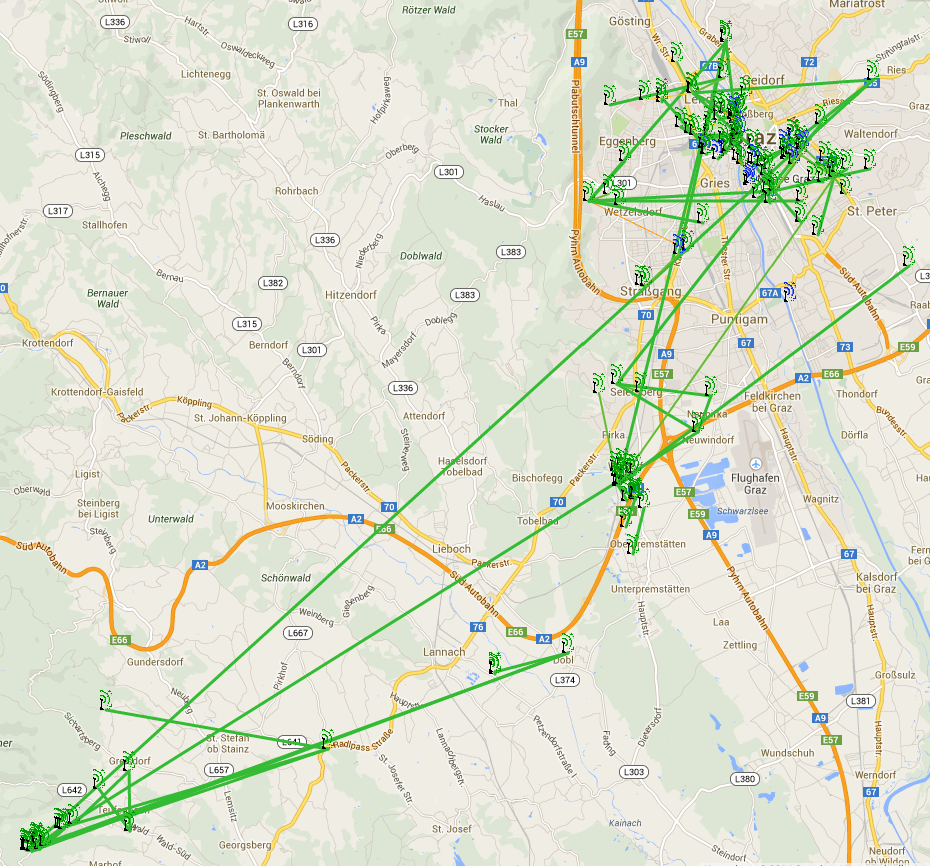
\includegraphics{images/graz_map.png}

\begin{longtable}[c]{@{}crrr@{}}
\toprule\addlinespace
Degree & Ninux & FFWien & FFGraz
\\\addlinespace
\midrule\endhead
1 & 69.02 & 77.96 & 64.72
\\\addlinespace
2 & 22.64 & 27.46 & 27.28
\\\addlinespace
3 & 16.34 & 36.38 & 18.80
\\\addlinespace
4 & 9.66 & 36.24 & 11.72
\\\addlinespace
5 & 4.36 & 18.34 & 2.04
\\\addlinespace
6 & 1.98 & 11.40 & 7.32
\\\addlinespace
7 & 1.00 & 8.50 & 2.80
\\\addlinespace
8 & 4.00 & 3.62 & 2.24
\\\addlinespace
9 & 2.00 & 4.62 & 1.84
\\\addlinespace
10 & 1.00 & 4.44 & 2.04
\\\addlinespace
11 & 0.00 & 1.98 & 1.24
\\\addlinespace
12 & 0.00 & 2.94 & 1.40
\\\addlinespace
13 & 0.00 & 0.46 & 0.28
\\\addlinespace
14 & 0.00 & 0.48 & 0.08
\\\addlinespace
15 & 0.00 & 1.18 & 0.28
\\\addlinespace
16 & 0.00 & 0.32 & 1.60
\\\addlinespace
17 & 0.00 & 0.50 & 0.00
\\\addlinespace
18 & 0.00 & 0.02 & 0.00
\\\addlinespace
19 & 0.00 & 1.30 & 0.00
\\\addlinespace
20 & 0.00 & 0.62 & 0.00
\\\addlinespace
21 & 0.00 & 0.06 & 0.00
\\\addlinespace
\bottomrule
\addlinespace
\caption{Average degree frequencies in the three WCNs, over 50 samples}
\end{longtable}

\begin{figure}[htbp]
\centering
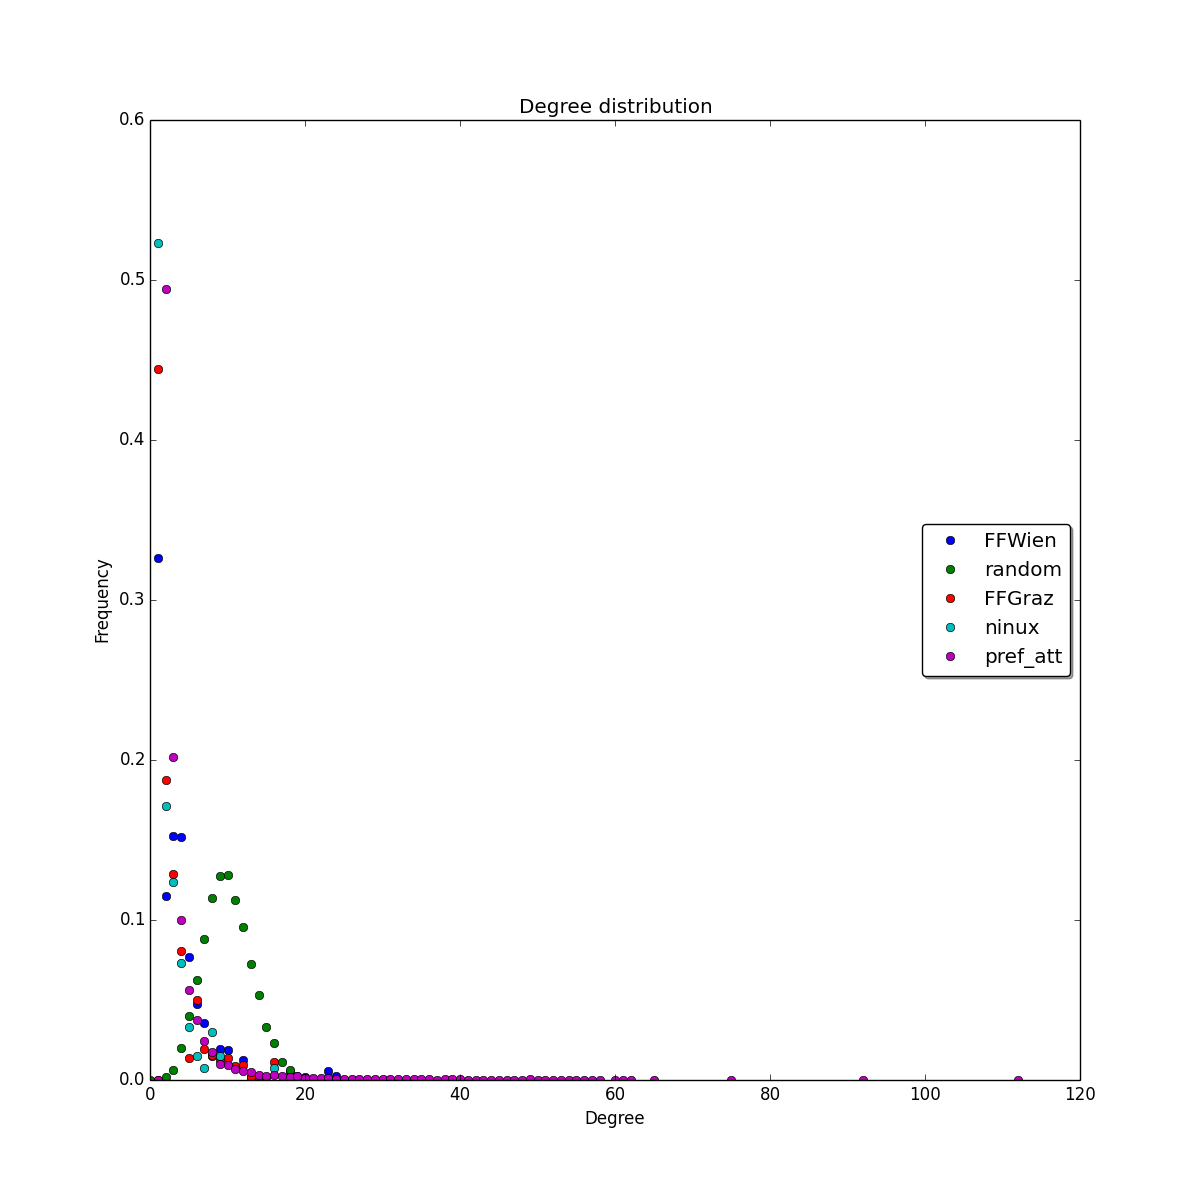
\includegraphics{synthetic_topologies/results/20140626-1629/degree_distribution.png}
\caption{Degree distributions of the three WCNs, compared with the
Erd\H{o}s-Rényi and Barabási-Albert models}
\end{figure}

\chapter{Robustness analysis}\label{robustness-analysis}

The first metric analysed is the robustness of the network. The chosen
methodology is a variation of the percolation process described in
Chapter 16 of (Newman 2010).

\section{Percolation}\label{percolation}

Percolation is the process of removing nodes (\emph{site percolation})
or edges (\emph{bond percolation}) and observing the properties of the
remaining graph. More specifically, by examining the connected
components of the graph, it can be decided if the underlying system is
still functioning the same after removing nodes (or edges). The removal
of nodes simulates a variety of real-world situations -- from hardware
failures in communication networks to vaccined people in the the spread
of a disease. Removing edges addresses other cases, also interesting in
real-world systems. In the following paragraphs, only site percolation
is considered, but the remarks are also valid, with the necessary
adaptations, for bond percolation.

It is not trivial, at a first look, how it should be decided if the
network ``functions'' after removing nodes. Nonetheless, there is a
simple answer to this issue that gives very significant results: the
order of the largest connected components. Removing a node from a
network obviously removes the node itself from any connected component,
but also affects potentially other nodes, which received information
through the removed node.

If enough nodes are removed, the network will become disconnected, but
usually there will be a large connected component containg most of the
surviving nodes and some smaller ones with just a few nodes. It can be
affirmed that in such a situation, at least part of the network is still
working as intended. Removing even more nodes, however, leads to a point
where the largest component does not contain a significat fraction of
the nodes -- it becomes indistinguishable from the smaller ones. This is
the point in which the network loses all its function.

To formally define a robustness metric, name the connected components of
a graph, ordered non-increasingly by the numer of their nodes,
$C_0, \ldots, C_m$. $|C_0|$ is then the order (number of nodes) of the
largest connected component. The robustness metric is defined as

\begin{equation}
S = \frac{|C_0|}{|V|}
\end{equation}

\section{Removal order}\label{removal-order}

Nodes and links in a network are not all equal. As seen in
\hyperref[networkux5ftopologyux5fandux5fgraphs]{Chapter 3}, different
centrality metrics give different measures of the importance of a node
in a network. When considering robustness, it is interesting to study
which nodes have the biggest impact when removed and how much difference
there is between more and less impacting nodes.

The classical approach to percolation is to remove nodes randomly in an
uniform way. Also popular is the removal of the nodes with highest
degree first. Other methods, such as ordering by centrality, have also
been explored. Comparing this different methods gives not only useful
information on how the metrics predict the impact of a node when
removed, but also on the behaviour of the examined networks. Some
networks, for example, behave more or less the same regardless of the
order of removal. Others show a dramatically different response.
Scale-free networks are the typical example of a network that is highly
robust to random failures, but collapses quickly if the nodes with the
highest degree are removed.

Changing the removal order has also another level of significance when
studying real-world networks. There are various situations in which
nodes have different probabilities of failing: for example, malicious
attacks often try to target the nodes that would cause the most damage.

All of the above considerations are also valid for links, but the
metrics differ: there is nothing corresponding to the degree, but there
is betweenness centrality.

This analysis covers random removal of both nodes and links, removal of
links by betweenness centrality and of nodes by degree, betweenness and
closeness centrality.

\section{Comparing different
networks}\label{comparing-different-networks}

The objective of doing a robustness analysis on WCNs, apart from
determining their resilience to failure, is also understanding if the
presently used random models are useful in describing their behaviour.

One feature of networks that highly influences their robustness is the
density of links with respect to nodes. Intuition suggests that a
network with more links should be more robust of a less dense one with
the same number of nodes. This is in fact confirmed.

Keeping this in mind, any robustness comparison between two networks is
significant if the networks have comparable densities. It is of no use
comparing a 100-node network with 200 edges to one with 2000.

To express the density of a graph, the average degree may be used.
Recall the three WCNs which are the subject of this analysis have
average degrees 2.333, 3.654 and 2.764. Since they are to be compared to
graphs generated by random models, care must be taken to generate graphs
with an averare degree not too distant from those.

The average degree of random graphs can be predicted easily, given the
parameters:

\begin{itemize}
\item
  for the Erd\H{o}s-Rényi $G(n,p)$ model, the expected average degree is

  \begin{equation}
  \left< k \right> = \frac{2 \binom{n}{2} p}{n} = (n-1)p
  \end{equation}
\item
  for the Barabási-Albert preferential attachment model the exact
  average degree is known

  \begin{equation}
  \left< k \right> = \frac{2 (n-m)m}{n} = 2m\left( 1 - \frac{m}{n} \right)
  \end{equation}
\end{itemize}

Unfortunately, while the $p$ parameter of the $G(n,p)$ model is a real
number and can be adjusted at will, the preferential attachment models
requires a natural number $m$. This means that only some values of
average degree can be achieved.

\begin{longtable}[c]{@{}ccccccc@{}}
\toprule\addlinespace
$m$ & 1 & 2 & 3 & 4 & 5 & 6
\\\addlinespace
$\left< k \right>$ & 1.99 & 3.96 & 5.91 & 7.84 & 9.75 & 11.64
\\\addlinespace
\bottomrule
\addlinespace
\caption{Average degrees for a 200-node graph with the Barabási-Albert
model}
\end{longtable}

\section{Methodology}\label{methodology}

The analysis was performed on 50 recent snapshots of the topology of the
three WCNs, as well as 30 graphs for each of the random models.

The algorithm simply removed nodes (or links) one by one and checked the
size of the largest connected component. In the case of random removal,
the test was repeated 30 times for each graph, changing the order every
time.

The test considered the removal of at most 40\% of the nodes (or links).
Other values have been tried, but this was determined to be sufficient
to observe the expected behaviour. Highest values just increased the
simulation time without adding useful information.

The results were averaged over the graphs of the same kind and
normalized over the fraction of removed nodes, rather then the number of
nodes, in order to compare them in the same graph.

\section{Results}\label{results}

\begin{figure}[htbp]
\centering
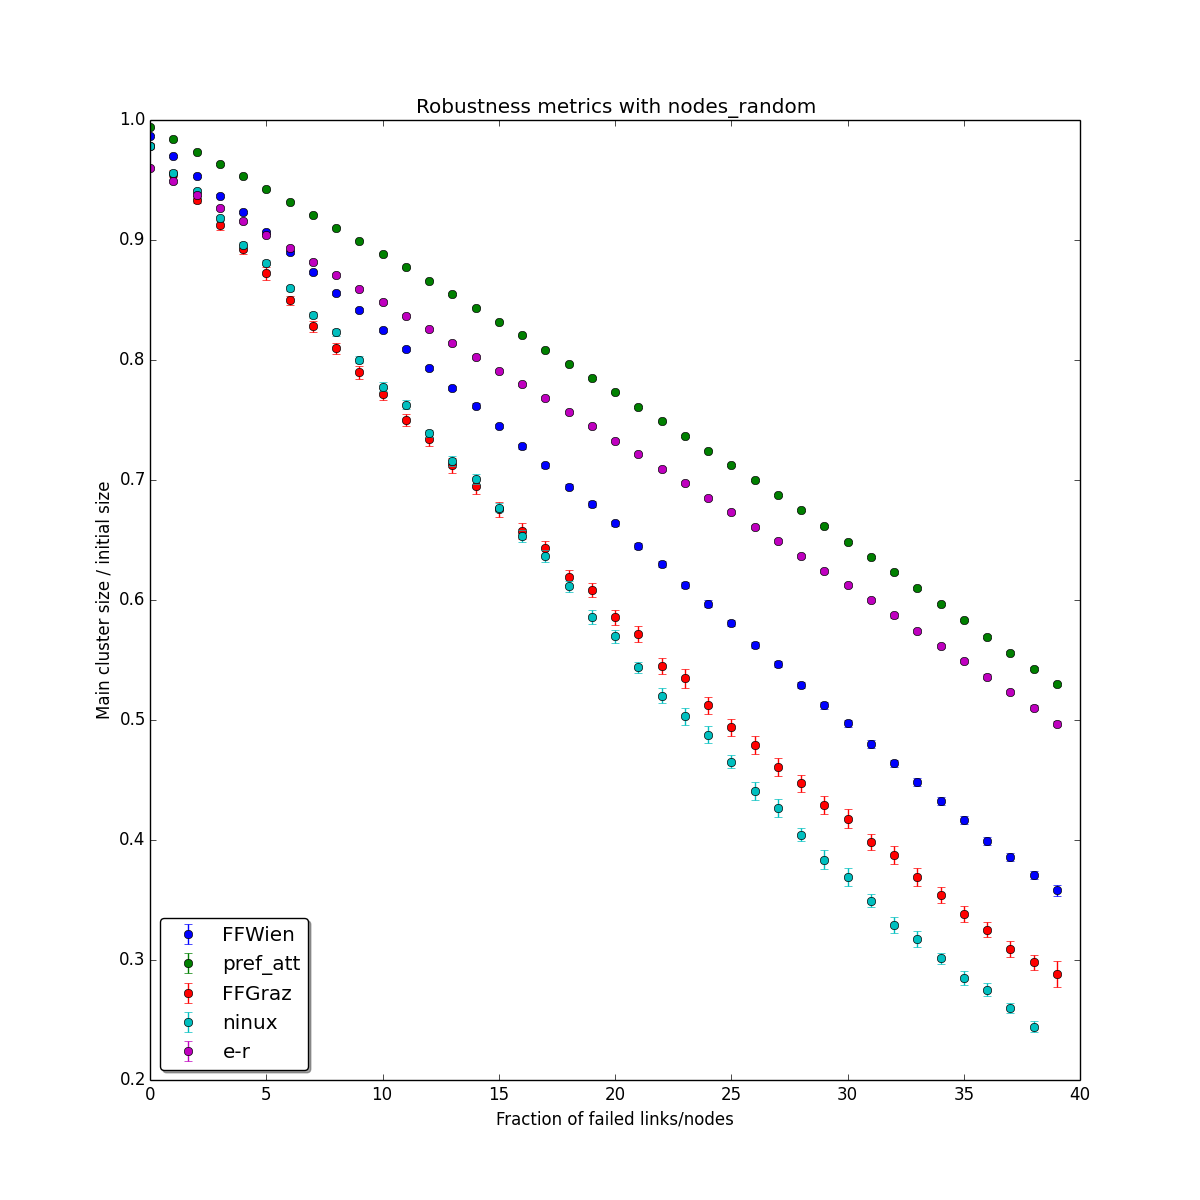
\includegraphics{./synthetic_topologies/results/20140618-1529/nodes_random_robustness.png}
\caption{Random removal}
\end{figure}

\begin{figure}[htbp]
\centering
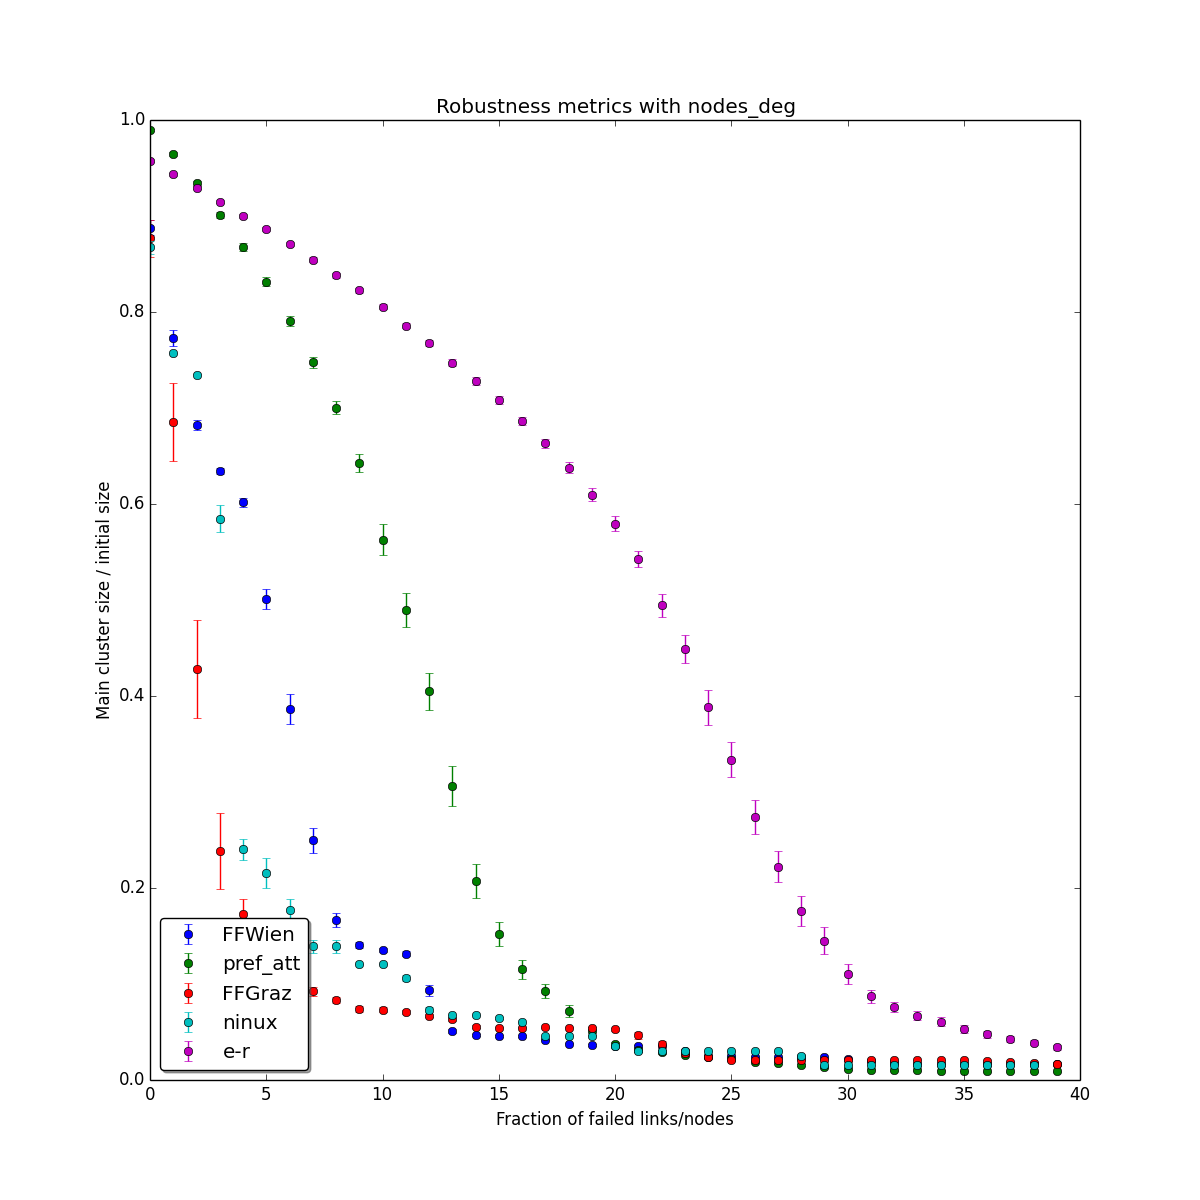
\includegraphics{./synthetic_topologies/results/20140618-1529/nodes_deg_robustness.png}
\caption{Removal by degree}
\end{figure}

\begin{figure}[htbp]
\centering
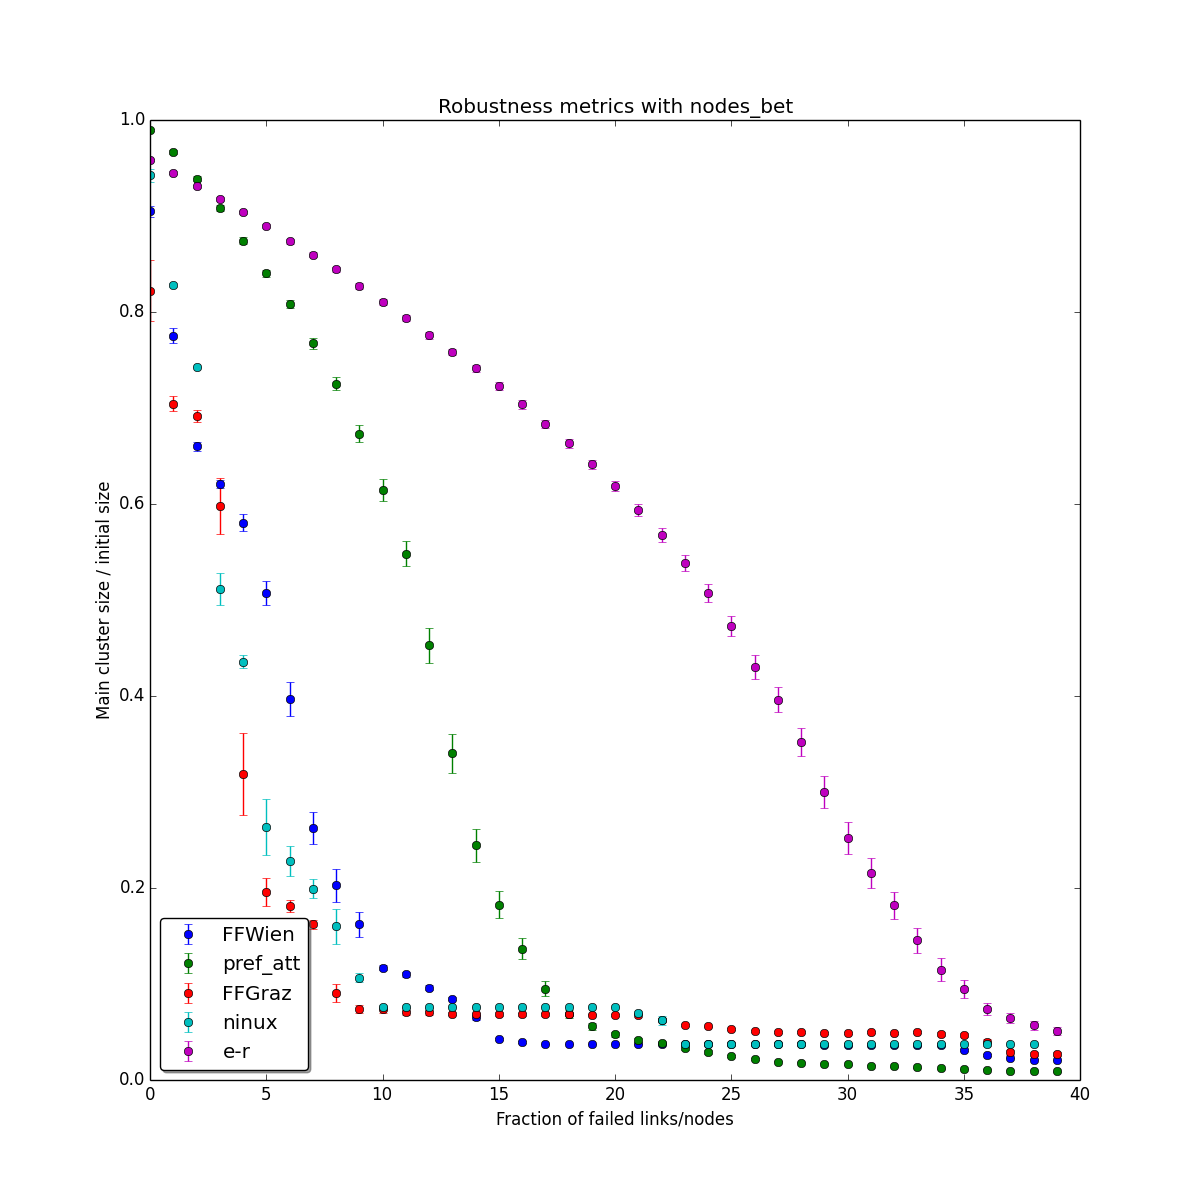
\includegraphics{./synthetic_topologies/results/20140618-1529/nodes_bet_robustness.png}
\caption{Removal by betweenness centrality}
\end{figure}

As shown in the figures, there is a marked difference between the
behaviour of the three WCNs (which is similar) and the behaviour of the
random graphs. The WCNs are more fragile in all tests, but while the
difference in the random removal case may be explained by the lower
density, in all of the ordered removal cases the consistently fail after
just the 10\% of removed nodes.

The scale-free random networks is, as expected, less robust than the
Erd\H{o}s-Rényi model in targeted attack to nodes with the highest
degree, and shows the same proceeding with removal by betweenness. On
the other hand, removing nodes by closeness centrality does not really
show a big difference between the two models.

WCNs, on the contrary, behave the same in all the scenarios in which
nodes are removed in order, independently from the metric used. This
suggest that, in those networks, the central nodes are the same for all
the metrics. This also means that the topology of WCNs, despite the big
similarity of the degree distribution, is different from the
preferential attachment model. Moreover, this difference seems to go in
the direction of less robustness.

The removal of links also shows a similar picture. None of the random
models approximates well the behaviour of the WCNs, which quickly fail
after a small fraction of links has been removed. Here a peculiar
behaviour appears in FFGraz: in this network, there are some nicely
connected areas that are geographically distant between themselves, so
there are some long links that provide connection between those
clusters. These long links are apparently (and intuitively) the ones
with the highest centrality, so the first to be removed.

\chapter{Message propagation
analysis}\label{message-propagation-analysis}

\subsection{The importance of routing}\label{the-importance-of-routing}

The robustness of a network is based on a static analysis of the
connectivity of the network graph when removing nodes or links. A
communication network, however, is a dynamic system where information
needs to move between nodes. Moreover, the decentralised nature of
computer networks means that the complete topology of the network is not
necessarily the topology used to transmit information, depending on the
routing protocol used for the network.

Given this, in order to understand the behaviour of a communication
network we need to study the behaviour of its routing protocol with
different underlying topologies. We are interested in the phase of
topology discovery, where each node receives information on the
existence of the other nodes in the network and (part of) the route to
reach them.

Topology discovery in link state routing protocols is usually performed
with each node flooding the network with some kind of link-state
advertisement message. The possible variations are the flooding policy
and the contents of the message. The most popular routing protocols used
in mesh networks behave as follows:

\begin{itemize}
\itemsep1pt\parskip0pt\parsep0pt
\item
  B.A.T.M.A.N. uses the simplest possible flooding (each node just
  performs a duplicate detection to avoid loops) and the advertisement
  message contains the sender address and a sequence number (for the
  duplicate detection)
\item
  OLSR employs a more sophisticated flooding mechanism based on MPRs and
  the advertisement message contains the whole neighbourhood of the
  sender
\item
  versions of OLSR used in practice usually force each node to be an
  MPR,\footnote{Maccari (2013)} thus having an hybrid behaviour with
  flooding as in B.A.T.M.A.N.
\end{itemize}

\subsection{Problem definition}\label{problem-definition}

The network is represented by a weighted graph $G=(V,E)$, where weights
represent the probability of losing a packet on each link (we use the
ETX metric of OLSR for this purpose).

Each node creates a message with information on its neighbourhood and
propagates it to each neighbour. Each node also propagates the message
it receives, with a simple duplicate detection based on the sender to
avoid loops.

Further iterations of the analysis will consider a subset of nodes
generating and propagating the messages and a different protocol for
loop avoidance.

Given the above situation, we define

\begin{quote}
$T_u = \forall v \in N .$ ``node $v$ has a route to node $u$''
\end{quote}

\begin{quote}
$R_u = \forall v \in N .$ ``node $u$ has a route to node $v$''
\end{quote}

Determine the probability of $T_u$ and $R_u$ for each node $u$ in the
graph.

\subsection{Methodology}\label{methodology-1}

The propagation of a message with duplicate detection can be simulated
with a Breadth First Search (BFS) over the graph. The most important
variation is that before traversing an edge a random number is generated
and compared to the packet loss probability of that link, to check if
the transmission succeeds. During the BFS, the simulation keeps track of
which nodes received the message and based on the content of the message
determines the couples of nodes which have a known route between
themselves. The search is repeated for every node as the starting point.
The union of the results is then used to verify $T_u$ and $R_u$.

The random simulation is run 1000 times to gather a significant figure
of the probability of $T_u$ and $R_u$.

The propagation for a node is as follows in pseudocode:

\paragraph{function propagate(Graph g, Node
u)}\label{function-propagategraph-g-node-u}

\begin{verbatim}
message_sender <- u
message_content <- neighbourhood_of(u)
q <- Queue()
route_knowledge <- set()
u.visited <- True
for v in u.neighbours append (u,v) to q
while q is not empty do
    pop (u,v) from q
    n <- random()
    if (not v.visited) and (n ≥ weight(u,v))
        v.visited <- True
        for i in message_content
            add (i,v) to route_knowledge
        for w in v.neighbours append (v,w) to q if w ≠ u
return route_knowledge
\end{verbatim}

The function is run for each node in the graph an the results are
collected.

\paragraph{function propagate\_all(Graph
g)}\label{function-propagateux5fallgraph-g}

\begin{verbatim}
rk <- set()
t, r <- array()
for u in g
    rk <- rk ∪ propagate(g, u)
for u in g
    if (u,v) ∈ rk ∀ node v ≠ u
        t[u] <- 1
    else
        t[u] <- 0
    if (v,u) ∈ rk ∀ node v ≠ u
        r[u] <- 1
    else
        r[u] <- 0
return t, r
\end{verbatim}

\paragraph{function run\_simulation(Graph g, Integer
n)}\label{function-runux5fsimulationgraph-g-integer-n}

\begin{verbatim}
pt, pr <- array()
for n times
    t, r <- propagate_all(g)
    pt += t                                % sum each element
    pr += r                                % "
divide each element of pt by n
divide each element of pr by n
return pt, pr
\end{verbatim}

\subsection{Rationale}\label{rationale}

The feasibility of calculating $T_u$ and $R_u$ exactly has been
evaluated. However, the computational complexity of this approach seems
very high and likely does not justify its use in place of the Monte
Carlo simulation.

Going into the details, the probability of a message propagating from
node $u$ to node $v$ is easily calculated by\ldots{} \sout{summing the
probabilities of success for every simple path between the two nodes.}
With this result for every possible destination $v1\ldots vn$ of a
message transmitted by $u$, it's theoretically possible to calculate
$T_u$ but it's not easy: the events ``reaching v1''\ldots{}``reaching
vn'' are not independent, so the probability of ``reaching every node''
is not the product of their probabilities.

For example, if $w$ is in any simple path from $u$ to $v$, the
probability of success between $u$ and $v$ changes if it is known that
node $w$ has been reached.

$P(v) = P(w) \cdot P(v|w) + P(\lnot w) \cdot P(v|\lnot w)$

The value of $P(v|w)$ and $P(v|\lnot w)$ is not so obvious:

\begin{itemize}
\itemsep1pt\parskip0pt\parsep0pt
\item
  $P(v|w)$ is the sum of the probabilities of the subpaths
  $w \rightarrow v$ for every simple path $u→v$
\item
  $P(v|\lnot w)$ is the sum of the probabilities of success for simple
  paths from $u$ to $v$ excluding the paths that contain $w$
\end{itemize}

This must be computed for every $w$ that appears in at least one simple
path $u \rightarrow v$. Again, this computation must be repeated for
every possible source-destination pair $u,v$.

\chapter{Conclusions}\label{conclusions}

\chapter*{Bibliography}\label{bibliography}
\addcontentsline{toc}{chapter}{Bibliography}

Barabási, Albert-László, and Réka Albert. 1999. ``Emergence of Scaling
in Random Networks.'' \emph{Science} 286 (5439): 509--12.
doi:\href{http://dx.doi.org/10.1126/science.286.5439.509}{10.1126/science.286.5439.509}.
\url{http://www.sciencemag.org/content/286/5439/509}.

Clausen, T., and Philippe Jacquet. 2003. ``Optimized Link State Routing
Protocol (OLSR).'' IETF. \url{http://tools.ietf.org/html/rfc3626}.

De Couto, Douglas {SJ}. 2004. ``High-Throughput Routing for Multi-Hop
Wireless Networks.'' PhD thesis, MIT.
\url{http://citeseerx.ist.psu.edu/viewdoc/download?doi=10.1.1.117.3059\&rep=rep1\&type=pdf}.

Gilbert, E. N. 1959. ``Random Graphs.'' \emph{The Annals of Mathematical
Statistics} 30 (4): 1141--44.
doi:\href{http://dx.doi.org/10.1214/aoms/1177706098}{10.1214/aoms/1177706098}.
\url{http://projecteuclid.org/euclid.aoms/1177706098}.

``List of Wireless Community Networks by Region. Wikipedia, the Free
Encyclopedia.'' 2014. June 10.
\url{https://en.wikipedia.org/w/index.php?title=List_of_wireless_community_networks_by_region\&oldid=612342893}.

Maccari, Leonardo. 2013. ``An Analysis of the Ninux Wireless Community
Network.'' In \emph{Wireless and Mobile Computing, Networking and
Communications (WiMob), 2013 IEEE 9th International Conference on},
1--7. IEEE.
\url{http://ieeexplore.ieee.org/xpls/abs_all.jsp?arnumber=6673332}.

Newman, Mark. 2010. \emph{Networks: An Introduction}. Oxford University
Press, USA.

\end{document}
